\documentclass[14pt]{extbook}
\usepackage{multicol, enumerate, enumitem, hyperref, color, soul, setspace, parskip, fancyhdr} %General Packages
\usepackage{amssymb, amsthm, amsmath, latexsym, units, mathtools} %Math Packages
\everymath{\displaystyle} %All math in Display Style
% Packages with additional options
\usepackage[headsep=0.5cm,headheight=12pt, left=1 in,right= 1 in,top= 1 in,bottom= 1 in]{geometry}
\usepackage[usenames,dvipsnames]{xcolor}
\usepackage{dashrule}  % Package to use the command below to create lines between items
\newcommand{\litem}[1]{\item#1\hspace*{-1cm}\rule{\textwidth}{0.4pt}}
\pagestyle{fancy}
\lhead{Progress Quiz 3}
\chead{}
\rhead{Version ALL}
\lfoot{3012-8528}
\cfoot{}
\rfoot{Summer C 2021}
\begin{document}

\begin{enumerate}
\litem{
Solve the quadratic equation below. Then, choose the intervals that the solutions belong to, with $x_1 \leq x_2$ (if they exist).\[ -14x^{2} +8 x + 4 = 0 \]\begin{enumerate}[label=\Alph*.]
\item \( x_1 \in [-17.37, -16.32] \text{ and } x_2 \in [17.17, 17.55] \)
\item \( x_1 \in [-12.56, -11.5] \text{ and } x_2 \in [4.13, 5.1] \)
\item \( x_1 \in [-2.22, -0.67] \text{ and } x_2 \in [0.3, 0.6] \)
\item \( x_1 \in [-0.56, 0.35] \text{ and } x_2 \in [0.84, 0.98] \)
\item \( \text{There are no Real solutions.} \)

\end{enumerate} }
\litem{
Factor the quadratic below. Then, choose the intervals that contain the constants in the form $(ax+b)(cx+d); b \leq d.$\[ 81x^{2} +63 x + 10 \]\begin{enumerate}[label=\Alph*.]
\item \( a \in [0.6, 1.3], \hspace*{5mm} b \in [15, 25], \hspace*{5mm} c \in [-2.1, 2.5], \text{ and } \hspace*{5mm} d \in [45, 47] \)
\item \( a \in [7.3, 10.1], \hspace*{5mm} b \in [-1, 10], \hspace*{5mm} c \in [8.6, 11.1], \text{ and } \hspace*{5mm} d \in [5, 11] \)
\item \( a \in [1.4, 4.9], \hspace*{5mm} b \in [-1, 10], \hspace*{5mm} c \in [26.6, 27.6], \text{ and } \hspace*{5mm} d \in [5, 11] \)
\item \( a \in [24.5, 28.4], \hspace*{5mm} b \in [-1, 10], \hspace*{5mm} c \in [2.7, 5.4], \text{ and } \hspace*{5mm} d \in [5, 11] \)
\item \( \text{None of the above.} \)

\end{enumerate} }
\litem{
Solve the quadratic equation below. Then, choose the intervals that the solutions $x_1$ and $x_2$ belong to, with $x_1 \leq x_2$.\[ 15x^{2} +38 x + 24 = 0 \]\begin{enumerate}[label=\Alph*.]
\item \( x_1 \in [-2.92, -2.14] \text{ and } x_2 \in [-0.68, -0.45] \)
\item \( x_1 \in [-4.68, -3.59] \text{ and } x_2 \in [-0.46, -0.32] \)
\item \( x_1 \in [-20.65, -19.41] \text{ and } x_2 \in [-18.09, -17.93] \)
\item \( x_1 \in [-6.19, -4.51] \text{ and } x_2 \in [-0.33, -0.22] \)
\item \( x_1 \in [-2.35, -0.81] \text{ and } x_2 \in [-1.29, -1.03] \)

\end{enumerate} }
\litem{
Write the equation of the graph presented below in the form $f(x)=ax^2+bx+c$, assuming  $a=1$ or $a=-1$. Then, choose the intervals that $a, b,$ and $c$ belong to.
\begin{center}
    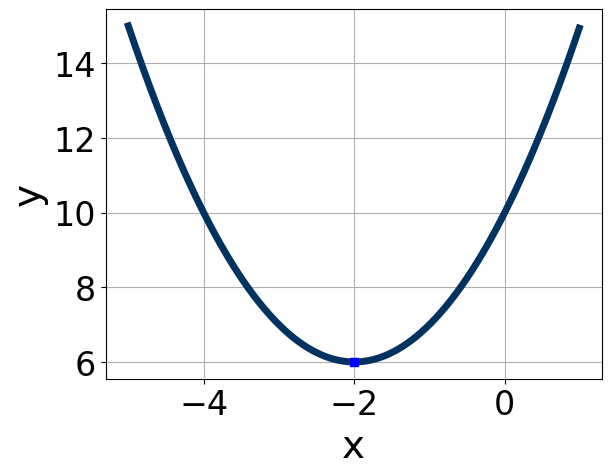
\includegraphics[width=0.5\textwidth]{../Figures/quadraticGraphToEquationCopyA.png}
\end{center}
\begin{enumerate}[label=\Alph*.]
\item \( a \in [0, 1.4], \hspace*{5mm} b \in [3, 5], \text{ and } \hspace*{5mm} c \in [9, 11] \)
\item \( a \in [0, 1.4], \hspace*{5mm} b \in [-4, 1], \text{ and } \hspace*{5mm} c \in [-2, 0] \)
\item \( a \in [0, 1.4], \hspace*{5mm} b \in [-4, 1], \text{ and } \hspace*{5mm} c \in [9, 11] \)
\item \( a \in [-1.2, -0.3], \hspace*{5mm} b \in [3, 5], \text{ and } \hspace*{5mm} c \in [0, 3] \)
\item \( a \in [-1.2, -0.3], \hspace*{5mm} b \in [-4, 1], \text{ and } \hspace*{5mm} c \in [0, 3] \)

\end{enumerate} }
\litem{
Graph the equation below.\[ f(x) = (x+4)^2 - 18 \]\begin{enumerate}[label=\Alph*.]
\begin{multicols}{2}\item 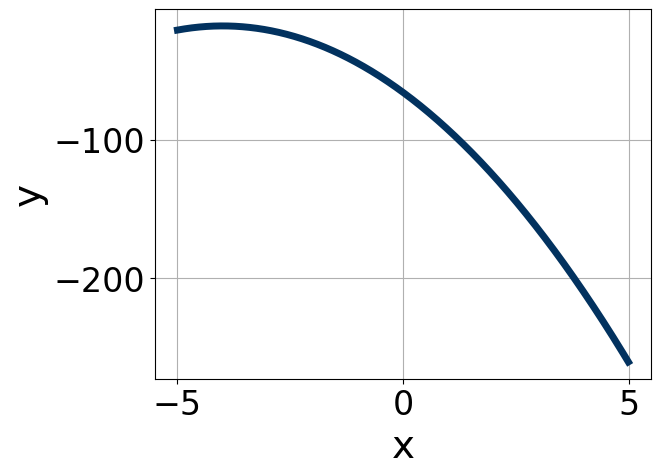
\includegraphics[width = 0.3\textwidth]{../Figures/quadraticEquationToGraphAA.png}\item 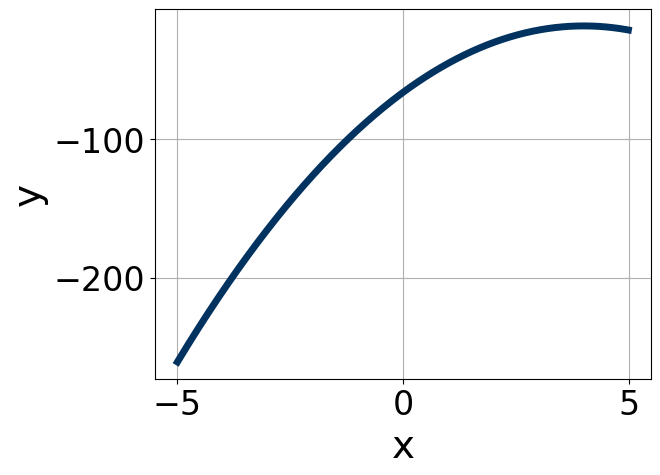
\includegraphics[width = 0.3\textwidth]{../Figures/quadraticEquationToGraphBA.png}\item 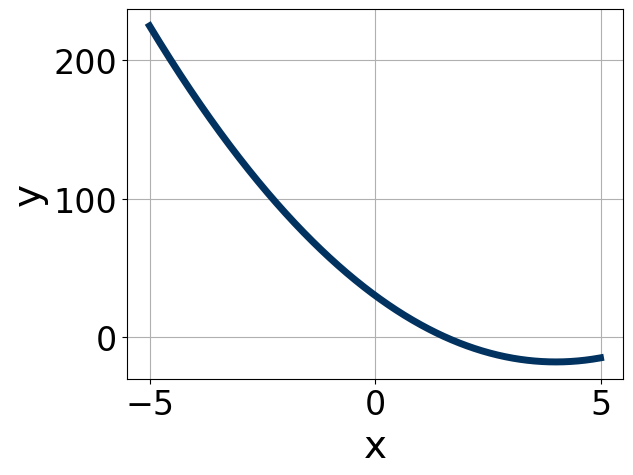
\includegraphics[width = 0.3\textwidth]{../Figures/quadraticEquationToGraphCA.png}\item 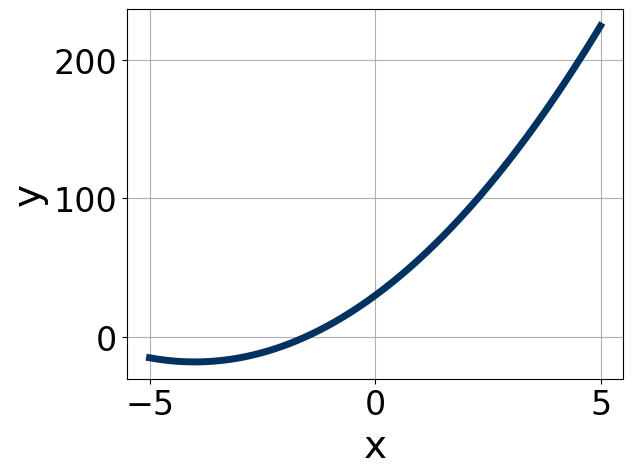
\includegraphics[width = 0.3\textwidth]{../Figures/quadraticEquationToGraphDA.png}\end{multicols}\item None of the above.
\end{enumerate} }
\litem{
Solve the quadratic equation below. Then, choose the intervals that the solutions $x_1$ and $x_2$ belong to, with $x_1 \leq x_2$.\[ 20x^{2} +21 x -54 = 0 \]\begin{enumerate}[label=\Alph*.]
\item \( x_1 \in [-9.03, -8.19] \text{ and } x_2 \in [0.16, 0.33] \)
\item \( x_1 \in [-7.24, -6.62] \text{ and } x_2 \in [0.31, 0.5] \)
\item \( x_1 \in [-3.06, -1.47] \text{ and } x_2 \in [1.19, 1.28] \)
\item \( x_1 \in [-45.82, -44.88] \text{ and } x_2 \in [23.87, 24.13] \)
\item \( x_1 \in [-1.66, -0.65] \text{ and } x_2 \in [3.46, 3.66] \)

\end{enumerate} }
\litem{
Factor the quadratic below. Then, choose the intervals that contain the constants in the form $(ax+b)(cx+d); b \leq d.$\[ 36x^{2} -60 x + 25 \]\begin{enumerate}[label=\Alph*.]
\item \( a \in [5.8, 7.1], \hspace*{5mm} b \in [-10, -3], \hspace*{5mm} c \in [3.5, 8.9], \text{ and } \hspace*{5mm} d \in [-8, -4] \)
\item \( a \in [0.3, 1.9], \hspace*{5mm} b \in [-30, -26], \hspace*{5mm} c \in [0.5, 2.4], \text{ and } \hspace*{5mm} d \in [-37, -24] \)
\item \( a \in [9.1, 15.3], \hspace*{5mm} b \in [-10, -3], \hspace*{5mm} c \in [2, 4.3], \text{ and } \hspace*{5mm} d \in [-8, -4] \)
\item \( a \in [1.1, 4.1], \hspace*{5mm} b \in [-10, -3], \hspace*{5mm} c \in [11, 13], \text{ and } \hspace*{5mm} d \in [-8, -4] \)
\item \( \text{None of the above.} \)

\end{enumerate} }
\litem{
Graph the equation below.\[ f(x) = (x+1)^2 - 17 \]\begin{enumerate}[label=\Alph*.]
\begin{multicols}{2}\item 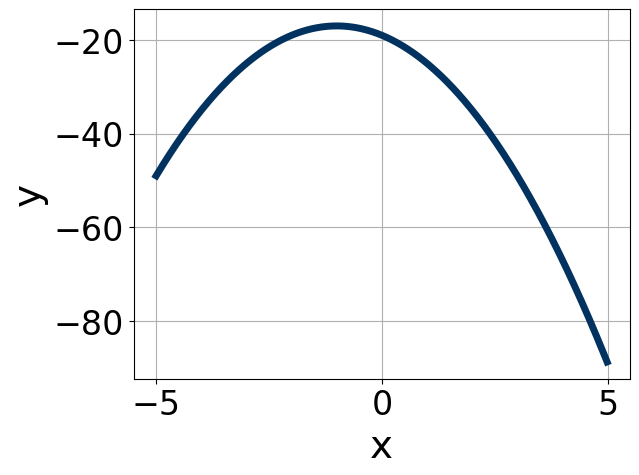
\includegraphics[width = 0.3\textwidth]{../Figures/quadraticEquationToGraphCopyAA.png}\item 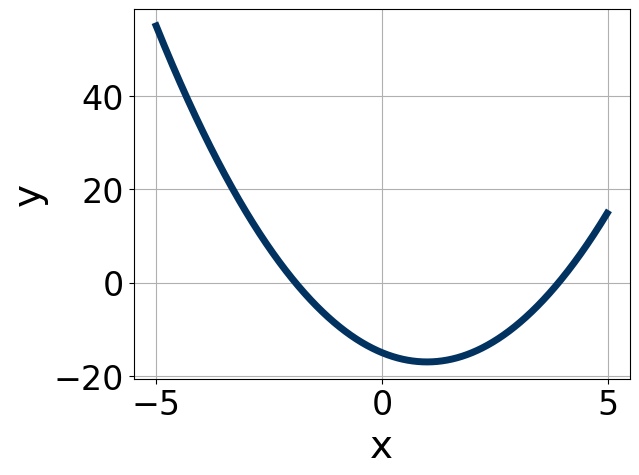
\includegraphics[width = 0.3\textwidth]{../Figures/quadraticEquationToGraphCopyBA.png}\item 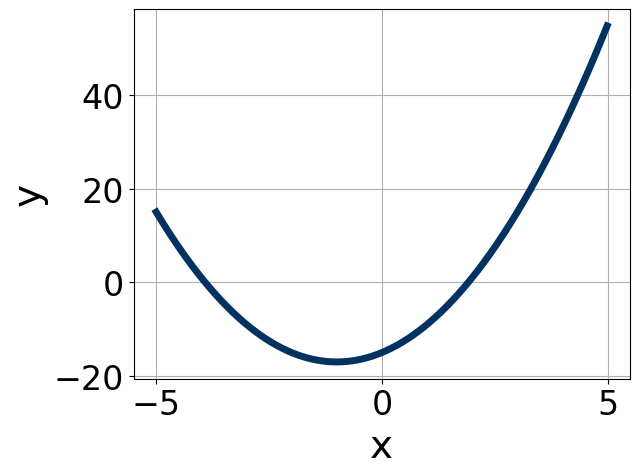
\includegraphics[width = 0.3\textwidth]{../Figures/quadraticEquationToGraphCopyCA.png}\item 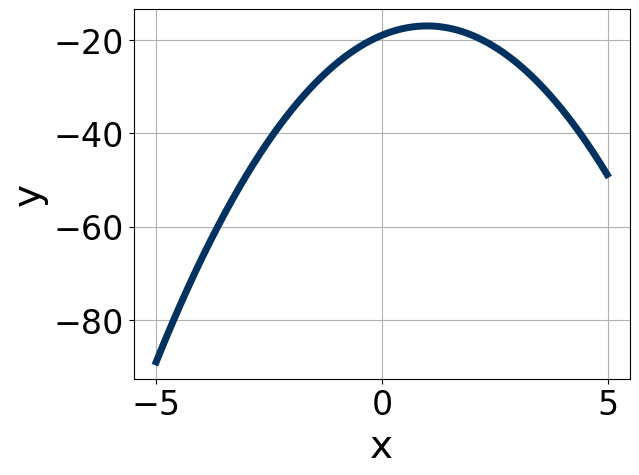
\includegraphics[width = 0.3\textwidth]{../Figures/quadraticEquationToGraphCopyDA.png}\end{multicols}\item None of the above.
\end{enumerate} }
\litem{
Solve the quadratic equation below. Then, choose the intervals that the solutions belong to, with $x_1 \leq x_2$ (if they exist).\[ 13x^{2} +14 x -2 = 0 \]\begin{enumerate}[label=\Alph*.]
\item \( x_1 \in [-0.8, 1.1] \text{ and } x_2 \in [0.93, 1.6] \)
\item \( x_1 \in [-16.6, -14.7] \text{ and } x_2 \in [1.66, 1.89] \)
\item \( x_1 \in [-3, -0.6] \text{ and } x_2 \in [-0.31, 0.41] \)
\item \( x_1 \in [-18, -16.5] \text{ and } x_2 \in [16.38, 17] \)
\item \( \text{There are no Real solutions.} \)

\end{enumerate} }
\litem{
Write the equation of the graph presented below in the form $f(x)=ax^2+bx+c$, assuming  $a=1$ or $a=-1$. Then, choose the intervals that $a, b,$ and $c$ belong to.
\begin{center}
    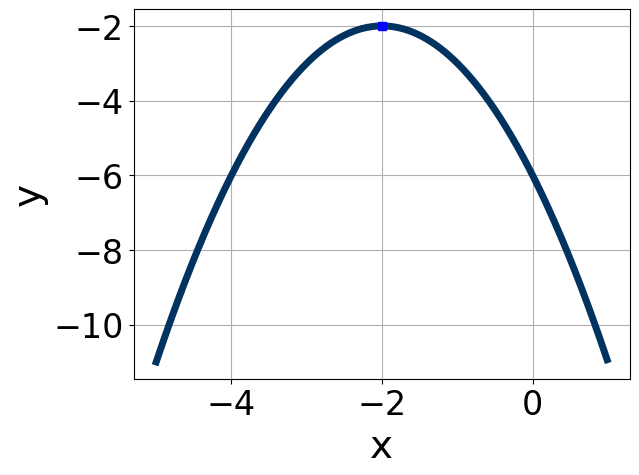
\includegraphics[width=0.5\textwidth]{../Figures/quadraticGraphToEquationA.png}
\end{center}
\begin{enumerate}[label=\Alph*.]
\item \( a \in [-0.2, 1.5], \hspace*{5mm} b \in [2, 6], \text{ and } \hspace*{5mm} c \in [2, 5] \)
\item \( a \in [-2.7, 0.9], \hspace*{5mm} b \in [-6, -2], \text{ and } \hspace*{5mm} c \in [-9, -5] \)
\item \( a \in [-0.2, 1.5], \hspace*{5mm} b \in [-6, -2], \text{ and } \hspace*{5mm} c \in [2, 5] \)
\item \( a \in [-2.7, 0.9], \hspace*{5mm} b \in [2, 6], \text{ and } \hspace*{5mm} c \in [-3, -1] \)
\item \( a \in [-2.7, 0.9], \hspace*{5mm} b \in [2, 6], \text{ and } \hspace*{5mm} c \in [-9, -5] \)

\end{enumerate} }
\litem{
Solve the quadratic equation below. Then, choose the intervals that the solutions belong to, with $x_1 \leq x_2$ (if they exist).\[ 10x^{2} -9 x -8 = 0 \]\begin{enumerate}[label=\Alph*.]
\item \( x_1 \in [-1.19, 0.09] \text{ and } x_2 \in [1, 3.1] \)
\item \( x_1 \in [-5.83, -5.41] \text{ and } x_2 \in [13.6, 15.8] \)
\item \( x_1 \in [-19.64, -19.51] \text{ and } x_2 \in [18.5, 21.1] \)
\item \( x_1 \in [-1.75, -0.97] \text{ and } x_2 \in [-0.5, 1.3] \)
\item \( \text{There are no Real solutions.} \)

\end{enumerate} }
\litem{
Factor the quadratic below. Then, choose the intervals that contain the constants in the form $(ax+b)(cx+d); b \leq d.$\[ 24x^{2} +2 x -15 \]\begin{enumerate}[label=\Alph*.]
\item \( a \in [7.29, 9.63], \hspace*{5mm} b \in [-3, 2], \hspace*{5mm} c \in [2.3, 3.5], \text{ and } \hspace*{5mm} d \in [3, 8] \)
\item \( a \in [3.77, 4.53], \hspace*{5mm} b \in [-3, 2], \hspace*{5mm} c \in [4.2, 7.7], \text{ and } \hspace*{5mm} d \in [3, 8] \)
\item \( a \in [1.92, 3.05], \hspace*{5mm} b \in [-3, 2], \hspace*{5mm} c \in [11.9, 14.9], \text{ and } \hspace*{5mm} d \in [3, 8] \)
\item \( a \in [0.51, 1.72], \hspace*{5mm} b \in [-26, -17], \hspace*{5mm} c \in [0.5, 1.3], \text{ and } \hspace*{5mm} d \in [17, 22] \)
\item \( \text{None of the above.} \)

\end{enumerate} }
\litem{
Solve the quadratic equation below. Then, choose the intervals that the solutions $x_1$ and $x_2$ belong to, with $x_1 \leq x_2$.\[ 25x^{2} -10 x -24 = 0 \]\begin{enumerate}[label=\Alph*.]
\item \( x_1 \in [-1.23, -0.61] \text{ and } x_2 \in [1.04, 1.36] \)
\item \( x_1 \in [-0.75, 0.1] \text{ and } x_2 \in [2.35, 2.99] \)
\item \( x_1 \in [-4.35, -2.85] \text{ and } x_2 \in [-0, 0.32] \)
\item \( x_1 \in [-20.19, -19.24] \text{ and } x_2 \in [29.63, 30.02] \)
\item \( x_1 \in [-1.97, -0.81] \text{ and } x_2 \in [0.36, 0.92] \)

\end{enumerate} }
\litem{
Write the equation of the graph presented below in the form $f(x)=ax^2+bx+c$, assuming  $a=1$ or $a=-1$. Then, choose the intervals that $a, b,$ and $c$ belong to.
\begin{center}
    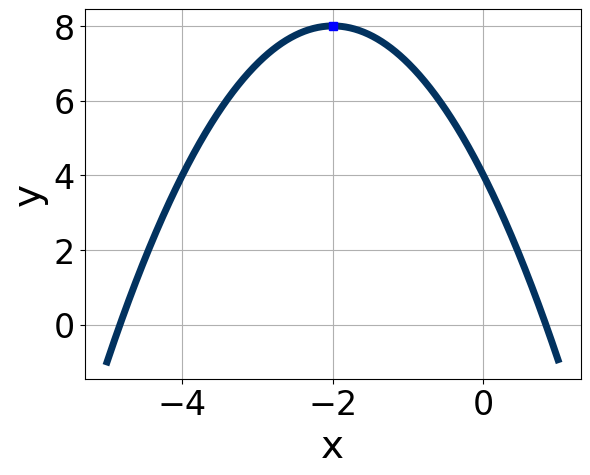
\includegraphics[width=0.5\textwidth]{../Figures/quadraticGraphToEquationCopyB.png}
\end{center}
\begin{enumerate}[label=\Alph*.]
\item \( a \in [0.7, 1.2], \hspace*{5mm} b \in [-5, -1], \text{ and } \hspace*{5mm} c \in [11, 14] \)
\item \( a \in [0.7, 1.2], \hspace*{5mm} b \in [1, 5], \text{ and } \hspace*{5mm} c \in [11, 14] \)
\item \( a \in [-1.6, -0.6], \hspace*{5mm} b \in [1, 5], \text{ and } \hspace*{5mm} c \in [2, 8] \)
\item \( a \in [-1.6, -0.6], \hspace*{5mm} b \in [-5, -1], \text{ and } \hspace*{5mm} c \in [2, 8] \)
\item \( a \in [-1.6, -0.6], \hspace*{5mm} b \in [1, 5], \text{ and } \hspace*{5mm} c \in [-12, -9] \)

\end{enumerate} }
\litem{
Graph the equation below.\[ f(x) = (x-3)^2 - 19 \]\begin{enumerate}[label=\Alph*.]
\begin{multicols}{2}\item 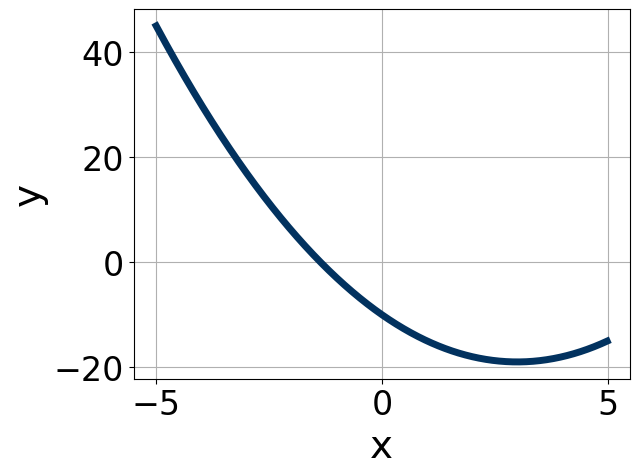
\includegraphics[width = 0.3\textwidth]{../Figures/quadraticEquationToGraphAB.png}\item 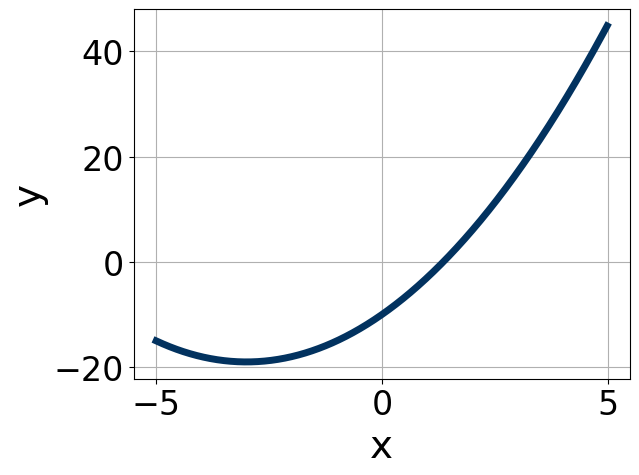
\includegraphics[width = 0.3\textwidth]{../Figures/quadraticEquationToGraphBB.png}\item 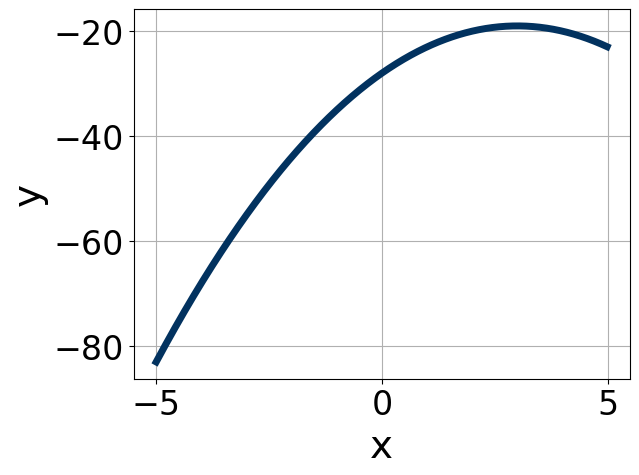
\includegraphics[width = 0.3\textwidth]{../Figures/quadraticEquationToGraphCB.png}\item 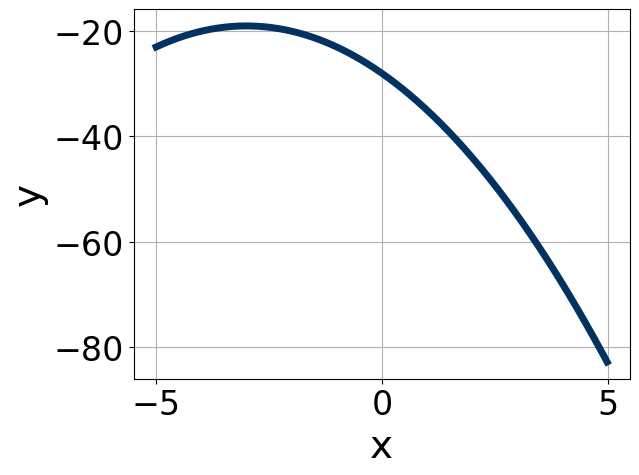
\includegraphics[width = 0.3\textwidth]{../Figures/quadraticEquationToGraphDB.png}\end{multicols}\item None of the above.
\end{enumerate} }
\litem{
Solve the quadratic equation below. Then, choose the intervals that the solutions $x_1$ and $x_2$ belong to, with $x_1 \leq x_2$.\[ 25x^{2} -10 x -24 = 0 \]\begin{enumerate}[label=\Alph*.]
\item \( x_1 \in [-0.53, -0.11] \text{ and } x_2 \in [2.39, 2.69] \)
\item \( x_1 \in [-4.11, -3.68] \text{ and } x_2 \in [0.03, 0.52] \)
\item \( x_1 \in [-1.71, -1.45] \text{ and } x_2 \in [0.31, 0.65] \)
\item \( x_1 \in [-0.87, -0.62] \text{ and } x_2 \in [1.01, 1.56] \)
\item \( x_1 \in [-20.08, -19.94] \text{ and } x_2 \in [29.98, 30.43] \)

\end{enumerate} }
\litem{
Factor the quadratic below. Then, choose the intervals that contain the constants in the form $(ax+b)(cx+d); b \leq d.$\[ 54x^{2} +15 x -25 \]\begin{enumerate}[label=\Alph*.]
\item \( a \in [1.7, 3.3], \hspace*{5mm} b \in [-9, -4], \hspace*{5mm} c \in [17.44, 18.8], \text{ and } \hspace*{5mm} d \in [5, 7] \)
\item \( a \in [-0.7, 2.4], \hspace*{5mm} b \in [-30, -22], \hspace*{5mm} c \in [0.21, 1.23], \text{ and } \hspace*{5mm} d \in [44, 48] \)
\item \( a \in [23.7, 27.8], \hspace*{5mm} b \in [-9, -4], \hspace*{5mm} c \in [1.83, 3.14], \text{ and } \hspace*{5mm} d \in [5, 7] \)
\item \( a \in [8.3, 10.3], \hspace*{5mm} b \in [-9, -4], \hspace*{5mm} c \in [5.77, 7.09], \text{ and } \hspace*{5mm} d \in [5, 7] \)
\item \( \text{None of the above.} \)

\end{enumerate} }
\litem{
Graph the equation below.\[ f(x) = -(x+4)^2 - 18 \]\begin{enumerate}[label=\Alph*.]
\begin{multicols}{2}\item 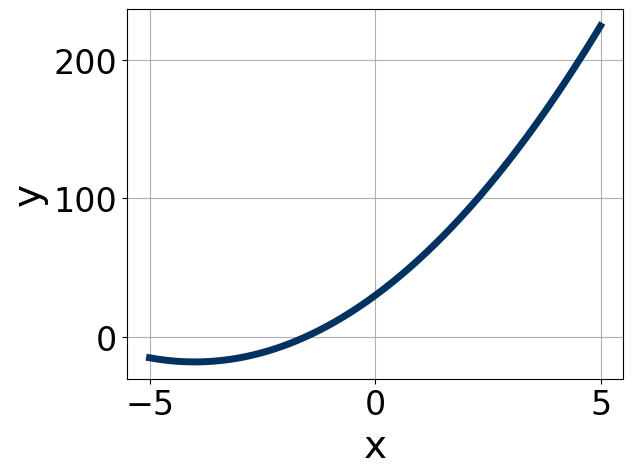
\includegraphics[width = 0.3\textwidth]{../Figures/quadraticEquationToGraphCopyAB.png}\item 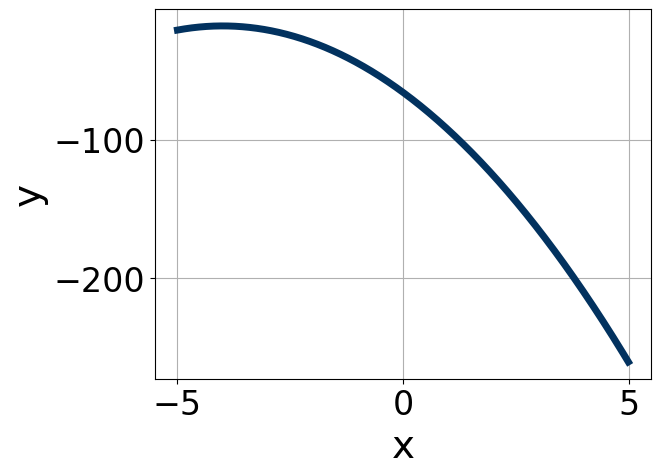
\includegraphics[width = 0.3\textwidth]{../Figures/quadraticEquationToGraphCopyBB.png}\item 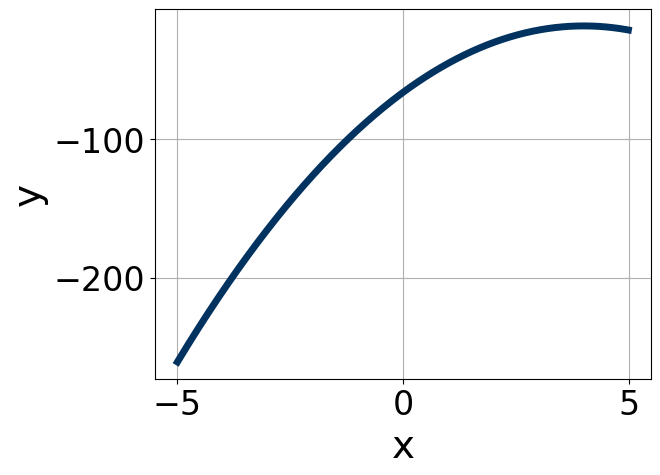
\includegraphics[width = 0.3\textwidth]{../Figures/quadraticEquationToGraphCopyCB.png}\item 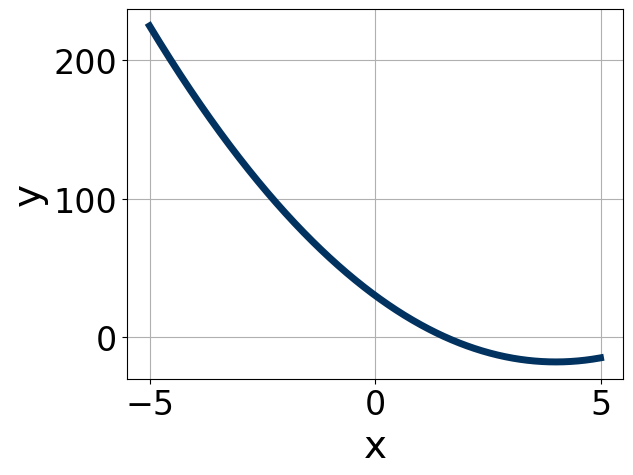
\includegraphics[width = 0.3\textwidth]{../Figures/quadraticEquationToGraphCopyDB.png}\end{multicols}\item None of the above.
\end{enumerate} }
\litem{
Solve the quadratic equation below. Then, choose the intervals that the solutions belong to, with $x_1 \leq x_2$ (if they exist).\[ 19x^{2} -13 x -5 = 0 \]\begin{enumerate}[label=\Alph*.]
\item \( x_1 \in [-6.3, -3.2] \text{ and } x_2 \in [17.66, 18.29] \)
\item \( x_1 \in [-23.7, -22.4] \text{ and } x_2 \in [23.22, 24.85] \)
\item \( x_1 \in [-1.7, -0.7] \text{ and } x_2 \in [0.21, 0.88] \)
\item \( x_1 \in [-0.5, 0.3] \text{ and } x_2 \in [0.8, 1.6] \)
\item \( \text{There are no Real solutions.} \)

\end{enumerate} }
\litem{
Write the equation of the graph presented below in the form $f(x)=ax^2+bx+c$, assuming  $a=1$ or $a=-1$. Then, choose the intervals that $a, b,$ and $c$ belong to.
\begin{center}
    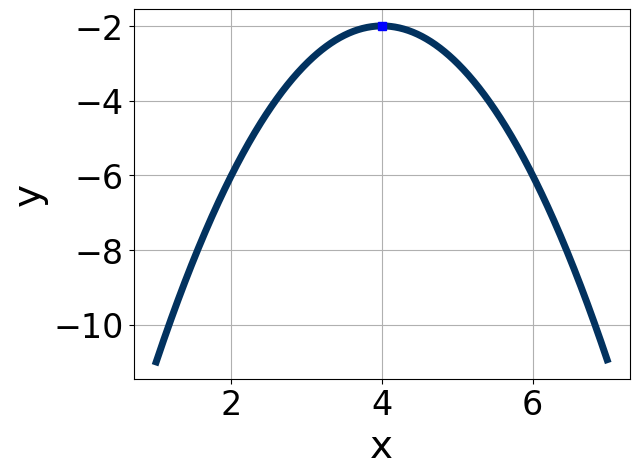
\includegraphics[width=0.5\textwidth]{../Figures/quadraticGraphToEquationB.png}
\end{center}
\begin{enumerate}[label=\Alph*.]
\item \( a \in [-1, 0], \hspace*{5mm} b \in [-8, -4], \text{ and } \hspace*{5mm} c \in [-18, -16] \)
\item \( a \in [0, 4], \hspace*{5mm} b \in [-8, -4], \text{ and } \hspace*{5mm} c \in [14, 16] \)
\item \( a \in [-1, 0], \hspace*{5mm} b \in [-8, -4], \text{ and } \hspace*{5mm} c \in [-16, -10] \)
\item \( a \in [0, 4], \hspace*{5mm} b \in [6, 9], \text{ and } \hspace*{5mm} c \in [14, 16] \)
\item \( a \in [-1, 0], \hspace*{5mm} b \in [6, 9], \text{ and } \hspace*{5mm} c \in [-18, -16] \)

\end{enumerate} }
\litem{
Solve the quadratic equation below. Then, choose the intervals that the solutions belong to, with $x_1 \leq x_2$ (if they exist).\[ -16x^{2} -15 x + 8 = 0 \]\begin{enumerate}[label=\Alph*.]
\item \( x_1 \in [-0.8, 0.6] \text{ and } x_2 \in [0.5, 2.9] \)
\item \( x_1 \in [-6.5, -5.4] \text{ and } x_2 \in [20.4, 23.1] \)
\item \( x_1 \in [-28.9, -26.1] \text{ and } x_2 \in [25.8, 28.3] \)
\item \( x_1 \in [-1.4, -1.2] \text{ and } x_2 \in [-0.1, 0.8] \)
\item \( \text{There are no Real solutions.} \)

\end{enumerate} }
\litem{
Factor the quadratic below. Then, choose the intervals that contain the constants in the form $(ax+b)(cx+d); b \leq d.$\[ 54x^{2} -69 x + 20 \]\begin{enumerate}[label=\Alph*.]
\item \( a \in [1.1, 2.9], \hspace*{5mm} b \in [-8, 1], \hspace*{5mm} c \in [26.7, 27.1], \text{ and } \hspace*{5mm} d \in [-5, 6] \)
\item \( a \in [4.8, 7.1], \hspace*{5mm} b \in [-8, 1], \hspace*{5mm} c \in [7, 10.5], \text{ and } \hspace*{5mm} d \in [-5, 6] \)
\item \( a \in [16.5, 18.1], \hspace*{5mm} b \in [-8, 1], \hspace*{5mm} c \in [2.1, 4.6], \text{ and } \hspace*{5mm} d \in [-5, 6] \)
\item \( a \in [-1, 1.9], \hspace*{5mm} b \in [-49, -44], \hspace*{5mm} c \in [-1.6, 1.9], \text{ and } \hspace*{5mm} d \in [-26, -22] \)
\item \( \text{None of the above.} \)

\end{enumerate} }
\litem{
Solve the quadratic equation below. Then, choose the intervals that the solutions $x_1$ and $x_2$ belong to, with $x_1 \leq x_2$.\[ 20x^{2} +21 x -54 = 0 \]\begin{enumerate}[label=\Alph*.]
\item \( x_1 \in [-45.86, -43.9] \text{ and } x_2 \in [24, 24.04] \)
\item \( x_1 \in [-2.93, -1.16] \text{ and } x_2 \in [1.15, 1.23] \)
\item \( x_1 \in [-9.52, -7.6] \text{ and } x_2 \in [0.23, 0.33] \)
\item \( x_1 \in [-7.78, -6.38] \text{ and } x_2 \in [0.32, 0.43] \)
\item \( x_1 \in [-1.46, 0.27] \text{ and } x_2 \in [2.34, 2.49] \)

\end{enumerate} }
\litem{
Write the equation of the graph presented below in the form $f(x)=ax^2+bx+c$, assuming  $a=1$ or $a=-1$. Then, choose the intervals that $a, b,$ and $c$ belong to.
\begin{center}
    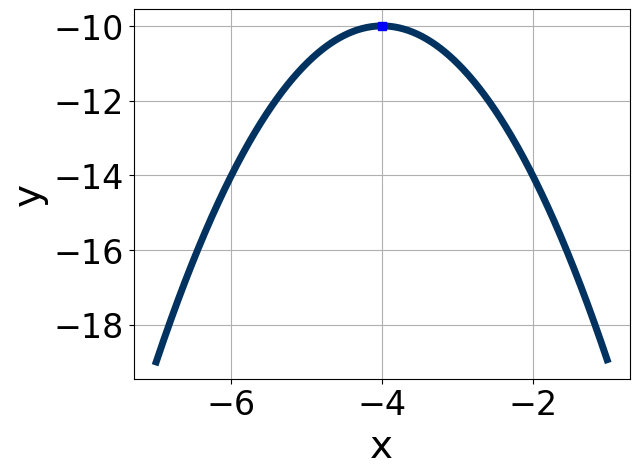
\includegraphics[width=0.5\textwidth]{../Figures/quadraticGraphToEquationCopyC.png}
\end{center}
\begin{enumerate}[label=\Alph*.]
\item \( a \in [-2.3, 0], \hspace*{5mm} b \in [7, 9], \text{ and } \hspace*{5mm} c \in [-29, -23] \)
\item \( a \in [-2.3, 0], \hspace*{5mm} b \in [-8, -5], \text{ and } \hspace*{5mm} c \in [-29, -23] \)
\item \( a \in [-0.8, 2], \hspace*{5mm} b \in [7, 9], \text{ and } \hspace*{5mm} c \in [5, 7] \)
\item \( a \in [-0.8, 2], \hspace*{5mm} b \in [-8, -5], \text{ and } \hspace*{5mm} c \in [5, 7] \)
\item \( a \in [-2.3, 0], \hspace*{5mm} b \in [7, 9], \text{ and } \hspace*{5mm} c \in [-9, 0] \)

\end{enumerate} }
\litem{
Graph the equation below.\[ f(x) = -(x-4)^2 - 20 \]\begin{enumerate}[label=\Alph*.]
\begin{multicols}{2}\item 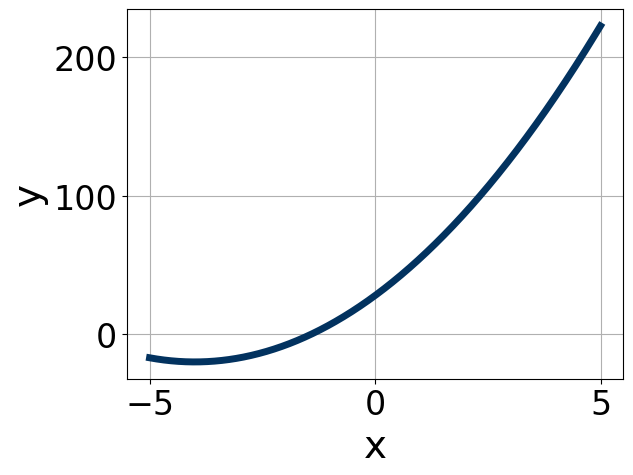
\includegraphics[width = 0.3\textwidth]{../Figures/quadraticEquationToGraphAC.png}\item 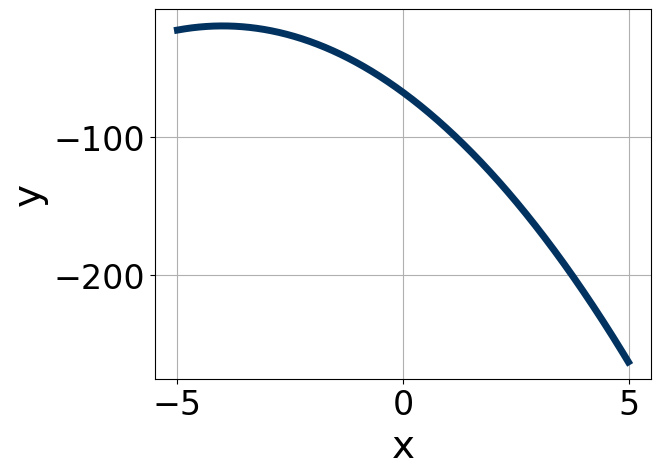
\includegraphics[width = 0.3\textwidth]{../Figures/quadraticEquationToGraphBC.png}\item 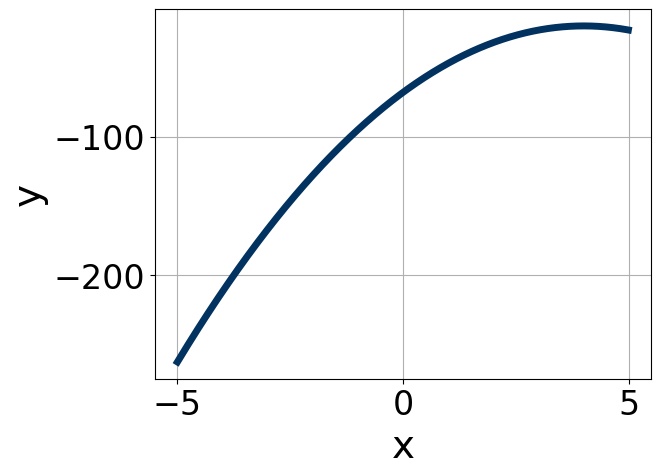
\includegraphics[width = 0.3\textwidth]{../Figures/quadraticEquationToGraphCC.png}\item 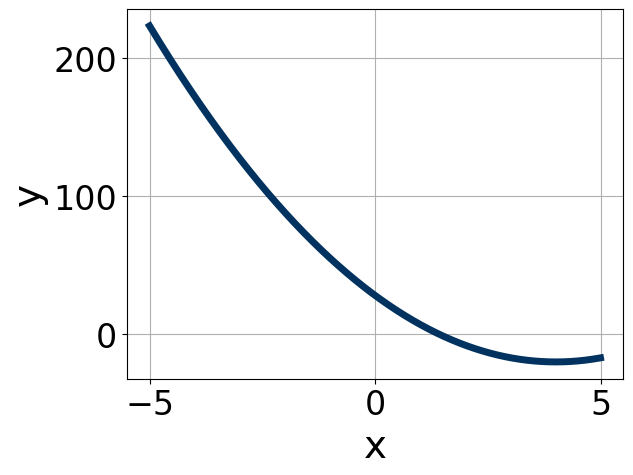
\includegraphics[width = 0.3\textwidth]{../Figures/quadraticEquationToGraphDC.png}\end{multicols}\item None of the above.
\end{enumerate} }
\litem{
Solve the quadratic equation below. Then, choose the intervals that the solutions $x_1$ and $x_2$ belong to, with $x_1 \leq x_2$.\[ 15x^{2} -38 x + 24 = 0 \]\begin{enumerate}[label=\Alph*.]
\item \( x_1 \in [17.89, 18.1] \text{ and } x_2 \in [19.88, 20.11] \)
\item \( x_1 \in [0.34, 0.59] \text{ and } x_2 \in [3.67, 4.24] \)
\item \( x_1 \in [1.15, 1.44] \text{ and } x_2 \in [1.18, 1.44] \)
\item \( x_1 \in [0.55, 0.63] \text{ and } x_2 \in [2.51, 2.95] \)
\item \( x_1 \in [0.66, 0.89] \text{ and } x_2 \in [2.33, 2.46] \)

\end{enumerate} }
\litem{
Factor the quadratic below. Then, choose the intervals that contain the constants in the form $(ax+b)(cx+d); b \leq d.$\[ 24x^{2} +38 x + 15 \]\begin{enumerate}[label=\Alph*.]
\item \( a \in [2.83, 5.18], \hspace*{5mm} b \in [-4, 5], \hspace*{5mm} c \in [5.75, 6.63], \text{ and } \hspace*{5mm} d \in [4, 6] \)
\item \( a \in [0.48, 1.02], \hspace*{5mm} b \in [14, 25], \hspace*{5mm} c \in [-0.66, 1.05], \text{ and } \hspace*{5mm} d \in [17, 21] \)
\item \( a \in [7.83, 8.35], \hspace*{5mm} b \in [-4, 5], \hspace*{5mm} c \in [2.9, 3.37], \text{ and } \hspace*{5mm} d \in [4, 6] \)
\item \( a \in [1.49, 2.68], \hspace*{5mm} b \in [-4, 5], \hspace*{5mm} c \in [10.76, 12.3], \text{ and } \hspace*{5mm} d \in [4, 6] \)
\item \( \text{None of the above.} \)

\end{enumerate} }
\litem{
Graph the equation below.\[ f(x) = -(x-4)^2 + 15 \]\begin{enumerate}[label=\Alph*.]
\begin{multicols}{2}\item 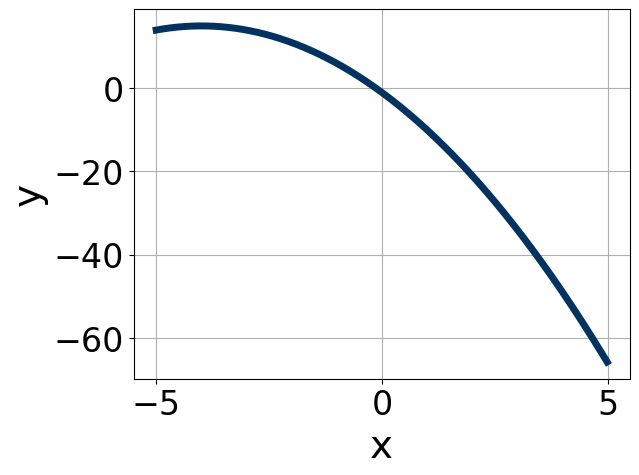
\includegraphics[width = 0.3\textwidth]{../Figures/quadraticEquationToGraphCopyAC.png}\item 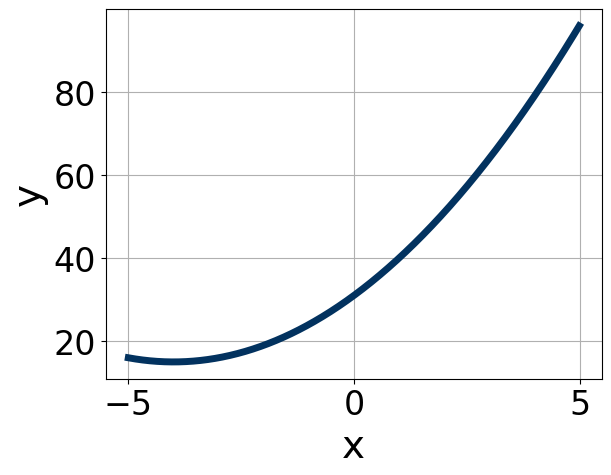
\includegraphics[width = 0.3\textwidth]{../Figures/quadraticEquationToGraphCopyBC.png}\item 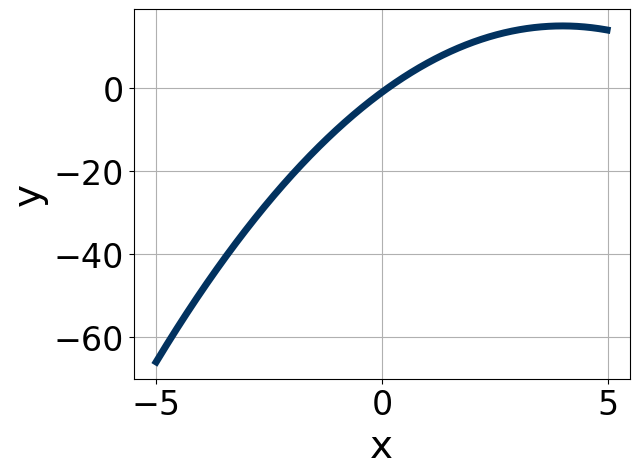
\includegraphics[width = 0.3\textwidth]{../Figures/quadraticEquationToGraphCopyCC.png}\item 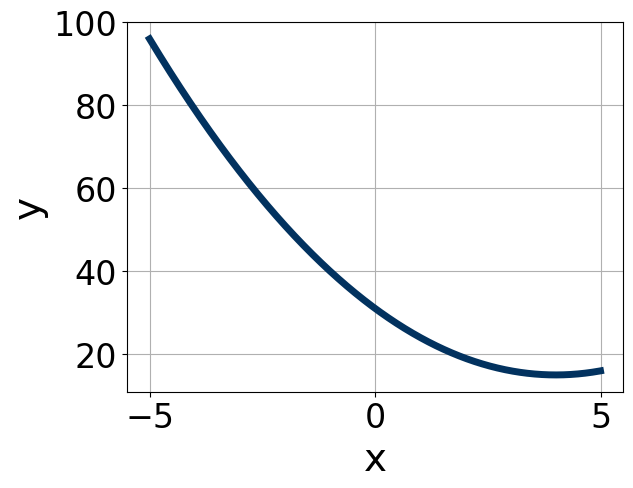
\includegraphics[width = 0.3\textwidth]{../Figures/quadraticEquationToGraphCopyDC.png}\end{multicols}\item None of the above.
\end{enumerate} }
\litem{
Solve the quadratic equation below. Then, choose the intervals that the solutions belong to, with $x_1 \leq x_2$ (if they exist).\[ 18x^{2} -9 x -6 = 0 \]\begin{enumerate}[label=\Alph*.]
\item \( x_1 \in [-1.49, -0.48] \text{ and } x_2 \in [-0.1, 0.46] \)
\item \( x_1 \in [-0.48, -0.37] \text{ and } x_2 \in [0.41, 1.42] \)
\item \( x_1 \in [-7.54, -6.59] \text{ and } x_2 \in [15.45, 16.28] \)
\item \( x_1 \in [-22.45, -21.84] \text{ and } x_2 \in [22.52, 23.78] \)
\item \( \text{There are no Real solutions.} \)

\end{enumerate} }
\litem{
Write the equation of the graph presented below in the form $f(x)=ax^2+bx+c$, assuming  $a=1$ or $a=-1$. Then, choose the intervals that $a, b,$ and $c$ belong to.
\begin{center}
    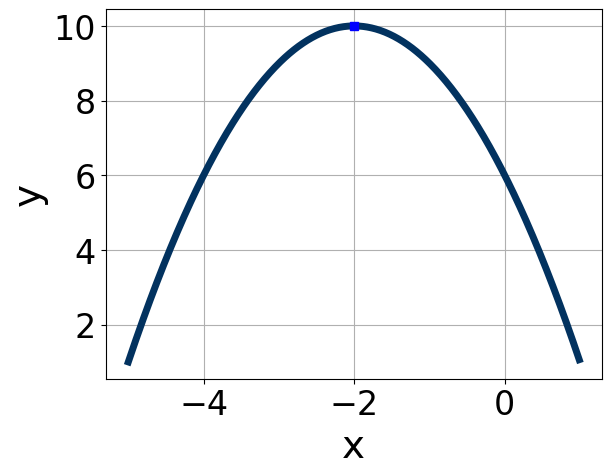
\includegraphics[width=0.5\textwidth]{../Figures/quadraticGraphToEquationC.png}
\end{center}
\begin{enumerate}[label=\Alph*.]
\item \( a \in [-1.1, -0.4], \hspace*{5mm} b \in [3, 6], \text{ and } \hspace*{5mm} c \in [-15, -10] \)
\item \( a \in [0.8, 2.9], \hspace*{5mm} b \in [3, 6], \text{ and } \hspace*{5mm} c \in [10, 15] \)
\item \( a \in [0.8, 2.9], \hspace*{5mm} b \in [-4, -1], \text{ and } \hspace*{5mm} c \in [10, 15] \)
\item \( a \in [-1.1, -0.4], \hspace*{5mm} b \in [-4, -1], \text{ and } \hspace*{5mm} c \in [4, 7] \)
\item \( a \in [-1.1, -0.4], \hspace*{5mm} b \in [3, 6], \text{ and } \hspace*{5mm} c \in [4, 7] \)

\end{enumerate} }
\end{enumerate}

\end{document}